\documentclass[10pt]{article}

\usepackage[latin1]{inputenc}
\usepackage{amsmath, amssymb, amsfonts, amsthm}
\usepackage{upgreek}
\usepackage{amsthm}
\usepackage{fullpage}
\usepackage{graphicx}
\usepackage{cancel}
\usepackage{subfigure}
\usepackage{mathrsfs}
\usepackage{outlines}
\usepackage[font={sf,it}, labelfont={sf,bf}, labelsep=space, belowskip=5pt]{caption}
\usepackage{hyperref}
% \usepackage{minted}
\usepackage{titling}
\usepackage{xifthen}
\usepackage{color}
\usepackage{listings}

\usepackage{fancyhdr}
\usepackage[title]{appendix}
\usepackage{float}

\usepackage{import}

\usepackage{bm}

\newcommand{\documenttitle}{Elastic Rod Networks}

\DeclareMathOperator{\tr}{tr}
\DeclareMathOperator{\sgn}{sgn}
\DeclareMathOperator{\sinc}{sinc}
\DeclareMathOperator{\rref}{rref}
\DeclareMathOperator{\cof}{cof}
\DeclareMathOperator*{\sym}{sym}

\DeclareMathOperator{\diag}{diag}
\DeclareMathOperator*{\argmax}{argmax}
\DeclareMathOperator*{\argmin}{argmin}
\newcommand{\defeq}{\vcentcolon=}
\renewcommand{\Re}{\operatorname{Re}} \renewcommand{\Im}{\operatorname{Im}}
\allowdisplaybreaks

\pagestyle{fancy}
\headheight 24pt
\headsep    12pt
\lhead{\documenttitle}
\rhead{\today}
\fancyfoot[C]{} % hide the default page number at the bottom
\lfoot{}
\rfoot{\thepage}
\renewcommand{\headrulewidth}{0.4pt}
\renewcommand\footrulewidth{0.4pt}
\providecommand{\abs}[1]{\lvert#1\rvert}
\providecommand{\norm}[1]{\lVert#1\rVert}
\providecommand{\normlr}[1]{\left\lVert#1\right\rVert}
\providecommand{\dx}{\, \mathrm{d}x}
% \providecommand{\vint}[2]{\int_{#1} \! #2 \, \mathrm{d}x}
% \providecommand{\sint}[2]{\int_{\partial #1} \! #2 \, \mathrm{d}A}
\renewcommand{\div}{\nabla \cdot}
\providecommand{\cross}{\times}
\providecommand{\curl}{\nabla \cross}
\providecommand{\grad}{\nabla}
\providecommand{\laplacian}{\bigtriangleup}
\providecommand{\shape}{\Omega}
\providecommand{\mesh}{\mathcal{M}}
\providecommand{\boundary}{\partial \shape}
\providecommand{\vint}[3][\x]{\int_{#2} \! #3 \, \mathrm{d}#1}
\providecommand{\sint}[3][\x]{\int_{#2} \! #3 \, \mathrm{d}A(#1)}
\providecommand{\lint}[3][\x]{\int_{#2} \! #3 \, \mathrm{d}s(#1)}
\providecommand{\pder}[2]{\frac{\partial #1}{\partial #2}}
\providecommand{\spder}[3]{\frac{\partial^2 #1}{\partial #2 \partial #3}}
\providecommand{\tder}[2]{\frac{\mathrm{d} #1}{\mathrm{d} #2}}
\providecommand{\evalat}[2]{\left.#1\right|_{#2}}
\renewcommand{\vec}[1]{{\bf #1}}

\providecommand{\tderatzero}[2]{\left.\frac{\mathrm{d} #1}{\mathrm{d} #2}\right|_{#2 = 0}}

\newcommand{\TODO}[1]{\textbf{****** {\bf{[#1]}} ******}}

\usepackage{prettyref}
\newrefformat{sec}{Section~\ref{#1}}
\newrefformat{tbl}{Table~\ref{#1}}
\newrefformat{fig}{Figure~\ref{#1}}
\newrefformat{chp}{Chapter~\ref{#1}}
\newrefformat{eqn}{\eqref{#1}}
\newrefformat{set}{\eqref{#1}}
\newrefformat{alg}{Algorithm~\ref{#1}}
\newrefformat{apx}{Appendix~\ref{#1}}
\newrefformat{prop}{Proposition~\ref{#1}}
\newcommand\pr[1]{\prettyref{#1}}

\def\normal{{\bf n}}
\def\n{\normal}
\def\a{\vec{a}}
\def\b{\vec{b}}
\def\d{\vec{d}}
\def\t{\vec{t}}
\def\x{\vec{x}}
\def\X{\vec{X}}
\def\y{\vec{y}}
\def\z{\vec{z}}
\def\u{\vec{u}}
\def\f{\vec{f}}
\def\w{\vec{w}}
\def\p{\vec{p}}
\def\r{\vec{r}}
\def\v{\vec{v}}
\def\e{\vec{e}}
\def\thvec{{\bm \theta}}
\def\ue{\vec{u}^\e}
\def\fu{\pder{\f}{u}}
\def\fv{\pder{\f}{v}}
\def\strain{\varepsilon}
\def\stress{\sigma}
\def\kb{\kappa \b}
\def\kbi{(\kappa \b)_i}
\def\k{\kappa}
\def\R{\, \mathbb{R}}
\def\L{\, \mathcal{L}}
\def\segment{s}
\def\joint{\jmath}

\providecommand\ts[1]{\widehat{\vec{t}^{#1}}}
\providecommand\ds[2]{\widehat{\vec{d}^{#1}_{#2}}}
\providecommand\rd[2]{\underline{\vec{d}^{#1}_{#2}}}
\providecommand\rds[2]{\widehat{\underline{\vec{d}^{#1}_{#2}}}}
\providecommand{\PXport}[1]{P_{\ts{#1}}^{\t^{#1}}}

\providecommand{\compose}{\circ}
\providecommand{\surface}{\Gamma}
\providecommand{\surfacegrad}{\nabla_\surface}
\providecommand{\surfacediv}{\surfacegrad \cdot}
\providecommand{\surfacelaplacian}{\laplacian_\surface}

\providecommand{\epssurface}{{\Gamma_\epsilon}}
\providecommand{\epssurfacegrad}{\nabla_\epssurface}
\providecommand{\epssurfacediv}{\epssurfacegrad \cdot}
\providecommand{\epsnormal}{\normal_\epsilon}
\providecommand{\epsnormalmat}{\tilde{\normal}_\epsilon}
\providecommand{\epsphi}{\phi_\epsilon}
\providecommand{\normalmatder}{\dot{\normal}}
\providecommand{\shapefunc}{{\bm \phi}}

\def\vt{\vec{v}_t}
\def\k{\kappa}

\newcommand*{\rom}[1]{\expandafter\@slowromancap\romannumeral #1@}
\newcommand{\RN}[1]{\textup{\uppercase\expandafter{\romannumeral#1}}}

\newtheorem{lemma}{Lemma}
\newtheorem{proposition}{Proposition}
\newtheorem{corollary}{Corollary}

\makeatletter
\usepackage{mathtools}
\newcases{mycases}{\quad}{%
  \hfil$\m@th\displaystyle{##}$}{$\m@th\displaystyle{##}$\hfil}{\lbrace}{.}
\makeatother

\setlength{\droptitle}{-50pt}
\title{\documenttitle}
\author{Julian Panetta}

% BEGIN DOCUMENT
\begin{document}
\maketitle

This document describes how to model the static equilibria of networks formed
by elastic rods connecting at deformable joints. Contrary to the rod linkages
also implemented in this repository, the rods meeting a joint in this model
are not allowed to pivot freely, and the joint stores some elastic energy.
We begin with the joint model from \cite{Perez2015}, and the elastic rod model is the one
from \cite{Bergou2010} (with corrected gradients/Hessians).

Once we have implemented the joint model, we will run experiments to validate
the accuracy of the displacements it computes against a volumetric
(tetrahedral) finite element simulation of analogous joint geometry. If the
accuracy is poor, we will attempt to invent a better joint model, either one
that is better physically motivated or that is data driven (fit to data
generated by the volumetric simulation).
If the model is accurate, we will use the network simulation in some higher-level
design or analysis tool. For instance, we might implement a homogenization tool
for determining the effective material properties of a metamaterial (periodic
microstructure) built from elastic rods.

\section{Rod Network Graph}
\begin{figure}[h]
    \centering
    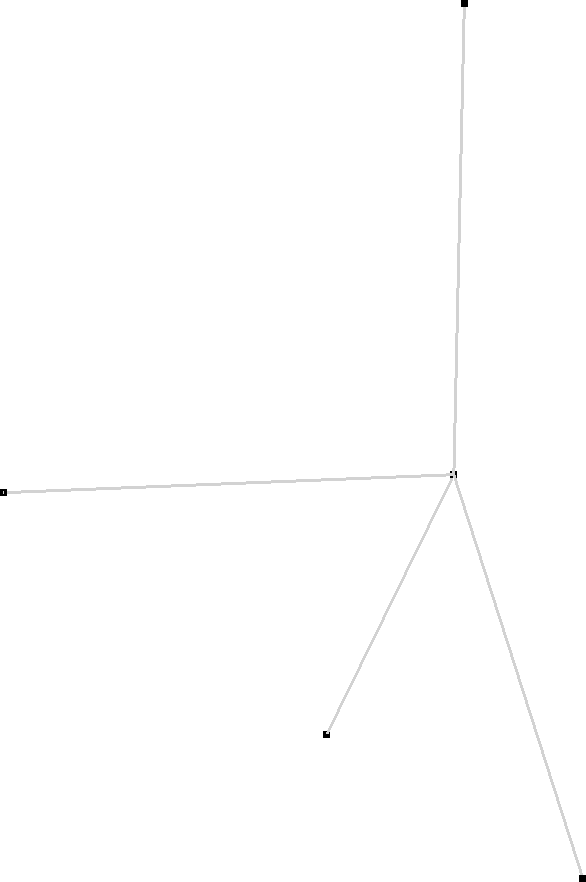
\includegraphics[width=.25\textwidth]{images/network_screenshot.png}
    \caption{An example rod network graph.}
    \label{fig:network_example}
\end{figure}
The network's initial configuration is defined by an embedded graph (i.e., line
mesh) with vertices and edges ($V$, $E$).
Each edge of this graph is referred to as a rod \emph{segment}. This embedded graph
is stored in the \texttt{OBJ} format using line elements (using the \texttt{l}
keyword instead of the usual \texttt{f}).

Each graph vertex represents either an elastic joint or a free rod end.

Each rod segment is modeled as a distinct discrete elastic rod with $n_s$
subdivisions (this includes up to 2 ``connection edges'' described above). We
label the $n^\text{th}$ segment $\segment_n$ for $n \in \{0\dots|E| - 1\}$ and
the joints $\joint_i$ for $i \in \{0\dots|J| - 1\}$, where $J \subset V$ is the
set of vertices of valence $2\text{--}4$.

\section{Rod and Joint Representation}
Recall that a discrete elastic rod's configuration is defined by its centerline positions
and its material frame angles (expressed relative to the rod's hidden reference
frame state). The material frame is used to express the orientation/twist of
the rod's cross sections, which is particularly important for flat, anisotropic
rods.

The network's rods meet at an elastic joint. Following \cite{Perez2015}, we define the
energy stored in the joint by constructing a fictitious ``connection edge'' for each incident elastic rod.
In the rest configuration, this connection edge continues straight across the joint (with the same tangent
and material axes as the terminal edge incident the joint).

Conceptually, all connection edges for a given joint behave as if they are
glued to a single rigid body at the joint. For a given deformed configuration
of the incident elastic rods, the orientation of this body is chosen to
approximately minimize the bending and twisting energy of the incident rods (by
solving the least-squares fitting in Eq (4) of \cite{Perez2015} and computing a
polar decomposition). Once this ``optimal'' rigid body orientation is found, it
determines the degrees of freedom of the connection edges (i.e., their
orientations and material axes). Applying this orientation to each connection
edge stores some twisting and bending energy in the incident rods; this energy
is defined to be the joint's energy.
TODO: draw a figure...

\section{Network Degrees of Freedom}
Our rod network model incorporates the constraints imposed by the joints by
constructing a reduced set of variables that parametrize all
admissible rod configurations. These reduced variables consist of (in order):
\begin{itemize}
    \item For each rod segment $\segment \in E$ :
    \begin{itemize}
        \item Centerline positions for all interior and free-end nodes of $s$.
            The $x$, $y$, and $z$ coordinates of the first interior/free node
            come first, followed by the coordinates for all subsequent
            nodes.
        \item Material frame angles $\theta$ for all interior and free-end edges of
              $\segment$.
    \end{itemize}
    \item The position of each joint $\joint \in J$.
\end{itemize}

\section{Elastic Energy, Gradients, and Hessians}
The elastic energy of the full network is computed by summing the energy from
each elastic rod and joint. However, because we implement the joint
energies by explicitly representing the ``connection edges'' in
the incident rod segments, the joint energy is effectively already contained in
the energy computed for the elastic rod segments. In other words, we only need
to sum the energy stored in each elastic rod segment.

We can then compute derivatives of this energy with respect to the degrees of
freedom by assembling the (transformed) derivatives of the discrete elastic rod
model.

\subsection{Gradients and Hessian}
First, we write the elastic energy with respect to the rod network's reduced variables
$$
E(\v(\r)),
$$
where vectors $\v$ and $\r$ collect the network's full and reduced variables.
By this, we mean $\v$ holds the full degrees of freedom of all elastic rods in
the network (including the variables controlling the connection edges), while
$\r$ holds only the non-connection edges' degrees of freedom and the joint
positions.

The gradient and Hessian with respect to the reduced variables are now given by the chain rule:
$$
\pder{E}{r_i} = \pder{E}{v_k}(\v(\r)) \pder{v_k}{r_i}
$$
$$
\spder{E}{r_i}{r_j} =
\pder{v_k}{r_i} \spder{E}{v_k}{v_l} \pder{v_l}{r_j}
+
\pder{E}{v_k} \spder{v_k}{r_i}{r_j}.
$$
The terms $\pder{v_k}{r_i}$ and $\spder{v_k}{r_i}{r_j}$ involve the gradients
and Hessians of the connection edge variables with respect to reduced
variables, which in turn involves the gradients and Hessians of the polar
decomposition.

\subsection{Practical Implementation Steps}
\begin{enumerate}
    \item Create the files \texttt{RodNetwork.\{hh,cc\}} by copying \texttt{RodLinkage.\{hh,cc\}}.
    \item Replace the existing \texttt{RodNetwork::Joint} class with one that supports an
        arbitrary number of incident rod segments (keeping track of which
        segments are incident and whether the joint appears at the beginning or
        end of the rod segment). This connectivity information can be stored in
        a pair of \texttt{std::vector}s. Most of the functions and data members
        brought over from \texttt{RodLinkage::Joint} should be removed (e.g.,
        the joint normal and constraint stuff; also the joint should only have
        its position as the degrees of freedom--eA and eB stuff should be
        removed).
    \item Write code to construct an elastic rod network from an OBJ file,
        building the elastic rod segments and joints based on the graph read from the file.
        The elastic rods should be built so that, for ends terminating in a
        joint, the last rod edge extends straight past the joint to form a
        ``connection edge.''

        Eventually, we will probably need an additional file that stores the
        orientation of material axis 1 (referred to as $\n$ in the rod
        mesh paper \cite{Perez2015} and $\d_1$ in \cite{Bergou2010} and the
        code) in the rest configuration for all rod endpoints appearing in a joint.
        This orientation cannot in general be inferred from the graph (though
        \cite{Perez2015} infers them with a heuristic that makes sense for
        networks lying on a surface, it doesn't make sense for ``volumetric''
        networks). For now, we can stick with rotationally-symmetric
        cross-sections, where this orientation is irrelevant.
        \texttt{RodNetwork::saveVisualizationGeometry} should be useful for
        debugging this step.
    \item Solve for the rigid transformation taking the fictitious rigid body
        at each joint from its rest configuration to its deformed configuration
        by performing the minimization in Eq (4) of \cite{Perez2015} and
        computing a polar decomposition. Debug this orientation by outputting
        an oriented cube for each joint (add a
        \texttt{RodNetwork::saveJointDebuggingGeometry}).
    \item Use this rigid transformation to orient the ``connection edges'' for
        each joint (transforming the first/last edges of the incident rod segments).
        At this point, the elastic energy of rod network should be computed properly.
    \item Update the \texttt{RodLinkage::gradient} to transform the individual
        elastic rod segment energy gradients using the chain rule and sum them
        into the full gradient. This chain rule involves the derivative of the polar
        decomposition as discussed in Eq (6) of \cite{Perez2015}.
        Validate the gradient using finite difference tests like in
        \texttt{test\_elastic\_rod\_linkage.cc}.
    \item Update the \texttt{RodLinkage::hessian} to transform the individual
        elastic rod segment energy Hessians and gradients using the chain rule and sum them
        into the full gradient. This chain rule involves the first and second derivatives of the polar
        decomposition; the latter is given in the appendix of \cite{Perez2015}.
        Validate the Hessian using finite difference tests like in
        \texttt{test\_elastic\_rod\_linkage.cc}.
\end{enumerate}

\subsection{Hessian Implementation Steps}
At a high level, the subtasks to complete are:
\begin{enumerate}
    \item Compute $\spder{D C^T}{u}{v}$ in \texttt{RodNetwork::Joint::d2\_DC\_dkdl} using the second
        derivative formulas for the tangent and normal vectors.
    \item Validate \texttt{RodNetwork::Joint::d2\_DC\_dkdl} by comparing against a finite
        difference of the matrices computed by \texttt{RodNetwork::Joint::DCdots}.
    \item Compute $\pder{S}{u}$ in \texttt{RodNetwork::Joint::Sdots} (should be relatively easy).
    \item Compute $\spder{R}{u}{v}$ in \texttt{RodNetwork::Joint::d2\_R\_dkdl} using the formulas for the second
        derivative of the polar decomposition. You will need to use the values computed by
        \texttt{RodNetwork::Joint::DCdots},
        \texttt{RodNetwork::Joint::d2\_DC\_dkdl},
        \texttt{RodNetwork::Joint::Sdots}, and 
        \texttt{RodNetwork::Joint::Rdots}.
    \item Validate \texttt{RodNetwork::Joint::d2\_R\_dkdl} by comparing against a finite
        difference of the matrices computed by \texttt{RodNetwork::Joint::Rdots}.
    \item Implement \texttt{RodNetwork::Joint::hessian}.
          This should be similar to the \texttt{RodNetwork::Joint::jacobian} implementation, except you need
          to use \texttt{d2\_R\_dkdl} instead of \texttt{d\_R\_dk}.
          You'll also need to use the product rule and the derivative of $\d_1$
          for the line that looks like:
          \begin{lstlisting}
Jac(3 * N + lsi, k) = -d_1.dot(d_R_dk[k] * rod.restMaterialFrameD2(edgeIdx));
          \end{lstlisting}
    \item Validate \texttt{RodNetwork::Joint::hessian} by comparing against a finite
        difference of the matrix \\
        \texttt{RodNetwork::Joint::jacobian}.
    \item Implement the chain rule expression for \texttt{RodNetwork::hessian} using 
        \texttt{RodNetwork::Joint::Rdots},
        \texttt{RodNetwork::Joint::d2\_R\_dkdl},
        \texttt{ElasticRod::hessian}, and
        \texttt{ElasticRod::gradient}. It may be helpful to read
        \texttt{RodLinkage::hessian}.
        
    \item Validate \texttt{RodNetwork::hessian} by comparing against a finite difference
        of \texttt{RodNetwork::gradient}.
\end{enumerate}

\subsection{Hessian representation}
The Hessian matrix of the elastic energy is quite large (it has as many rows and
columns as variables in the network), but most of its entries are 0. To
store the matrix efficiently, we use a sparse representation. Specifically, when constructing
the Hessian, we use a ``sparse triplet'' representation which simply stores
a large list of the row index, column index, and value of each nonzero entry
($(i, j, v)$ ``triplets''). Its fine to have multiple entries with the same row
and column index in this list: their values will be summed together to produce
the final sparse matrix. This fact will be useful when implementing all the
sums in the chain rule \pr{eqn:hessian_chain_rule} below (we can just push all
the values summing to a given $(i, j)$ entry into the list, and they will be
automatically summed for us at the end).

This sparse triplet representation is implemented by the \texttt{TMatrix} type,
which has inside it a \texttt{std::vector} named \texttt{nz} holding the
matrix's nonzero entries.

\subsection{Chain rule implementation}
Now let's look at how to implement the two terms appearing in the Hessian's chain rule:
$$
\spder{E}{r_i}{r_j} =
\pder{v_k}{r_i} \spder{E}{v_k}{v_l} \pder{v_l}{r_j}
+
\pder{E}{v_k} \spder{v_k}{r_i}{r_j}.
$$
First, we rewrite this Hessian in terms of a sum over the segments, since
the network's elastic energy is the sum of the elastic energy stored in each
segment:
\begin{equation}
\label{eqn:hessian_chain_rule}
    \spder{E}{r_i}{r_j} = \sum_s \left(
\pder{v^s_k}{r_i} \spder{E^s}{v^s_k}{v^s_l} \pder{v^s_l}{r_j}
+
\pder{E^s}{v^s_k} \spder{v^s_k}{r_i}{r_j}
    \right).
\end{equation}
Now $\pder{v^s_k}{r_i}$ is the Jacobian of segment $s$'s variables (i.e. red
and blue vertex/edge quantities) with respect to all the variables of the
network. This is a large sparse matrix with identity blocks for
the blue/joint quantities' rows and with entries from the \texttt{RodNetwork::Joint::jacobian}
matrix in the red quantities' rows. We already effectively
used this matrix to implement the \texttt{RodNetwork::gradient},
but we didn't explicitly construct it (we just implemented the matrix
multiplication it appeared in by using the entries we knew to be identity
blocks and the entries we knew came from \texttt{RodNetwork::Joint::jacobian}),
and won't construct it to build the Hessian either.
Tensor $\spder{v^s_k}{r_i}{r_j}$ is the Hessian of segment $s$'s variables
with respect to all the variables of the network---the nonzero
entries of this large matrix will come from \texttt{RodNetwork::Joint::hessian}.

Matrix $\spder{E^s}{v^s_k}{v^s_l}$ is the Hessian of segment $s$'s elastic
energy, which can be computed just by calling \texttt{ElasticRod::hessian}. This is
a sparse matrix in the sparse triplet format described above. To implement
the first term of the Hessian chain rule \pr{eqn:hessian_chain_rule},
you should loop over the nonzero entries stored in this triplet matrix's
\texttt{nz} array. Each of these entries gives you row and column indices---we'll call them
$k$ and $l$ here---as well as the element's value. This rod energy Hessian entry will contribute a whole list
of nonzero entries to the network energy Hessian:
for each $(i, j)$ such that $\pder{v^s_k}{r_i}$ and $\pder{v^s_l}{r_j}$ are nonzero,
you will add an $(i, j)$ entry to the network Hessian with value
$
\spder{E^s}{v^s_k}{v^s_l} * \pder{v^s_k}{r_i} \pder{v^s_l}{r_j}
$.
Essentially, this is just the sparse outer product of the vectors $\pder{v^s_k}{r_i}$ and $\pder{v^s_l}{r_j}$
(these are vectors because indices k and l are fixed) multiplied by the current entry of the rod energy Hessian.

To implement the second term of \pr{eqn:hessian_chain_rule}, you can loop over
the pairs $(i, j)$ of indices of network variables influencing either
the start or end joint of the current segment
(entries from \texttt{RodNetwork::jointVars}). For each of these $(i, j)$, you
find the $k$ indices for which
$\spder{v^s_k}{r_i}{r_j}$ is nonzero (this should just be the red vertices/edge
variables of the current segment's joints). Then, for each of these $k$, you
multiply the derivative of the segment's rod energy with respect to variable
$k$ (an entry from the \texttt{ElasticRod::gradient})
by the nonzero entry $\spder{v^s_k}{r_i}{r_j}$ (an entry from
\texttt{RodNetwork::hessian}) to obtain an output value for entry $(i, j)$ in
the network's Hessian.

\subsection{Computing $\spder{\t}{u}{v}$ and $\spder{\d_2}{u}{v}$}
To compute $\spder{DC^T}{u}{v}$ for a particular joint, we mainly
need to evaluate $\spder{\t}{u}{v}$ and $\spder{\d_2}{u}{v}$ for each blue edge
incident the joint. We do this by differentiating $\pder{\t}{u}$ and
$\pder{\d_2}{u}$ with respect to another of the joint's variables, $v$. We'll
get different expressions depending on the types of variables $u$ and $v$
(whether they are vertex coordinates or $\theta$s).

\subsubsection{Case 1: $u$ and $v$ both vertex coordinates}
We first consider the case where both variables control vertex
coordinates--either a coordinate of a blue vertex or the joint position.
In this case the derivatives with respect to $u$ are:
\begin{equation}
\label{eqn:grad_vtx_coord}
\begin{aligned}
      \pder{\t}{u} &= s_u \frac{I[:, u] - \t \, \t[u]}{\norm{\e}}
\\
    \pder{\d_2}{u} &= s_u \left[
            \frac{(\ds{}{1} \cdot \t) \left(\ts{} \cross \pder{\t}{u}\right) + (\ts{} \cross \t)\left(\ds{}{1} \cdot \pder{\t}{u}\right)}{1 + \ts{} \cdot \t}
          - \frac{(\ds{}{1} \cdot \t)(\ts{} \cross \t) \left(\ts{} \cdot \pder{\t}{u}\right)}{(1 + \ts{} \cdot \t)^2}
          - \ds{}{1} \cross \pder{\t}{u}
      \right],
\end{aligned}
\end{equation}
where $I[:, u]$ means the $u^\text{th}$ column of the $3\times3$ identity matrix,
and we've defined the sign multiplier:
$$
s_i =
\begin{mycases}
    \text{\texttt{orientation\_case}}  & \text{if $i$ is a joint position variable of the current segment} \\
    \text{-\texttt{orientation\_case}} & \text{if $i$ is a blue vertex position variable of the current segment} \\
    \text{0}                           & \text{otherwise}
\end{mycases}.
$$
Now, we can differentiate with respect to $v$, starting with $\t$:
\begin{align*}
    \spder{\t}{u}{v} &= s_u \left[ -s_v \frac{I[:, u] - \t \, \t[u]}{\norm{\e}^2} \t[v] - s_v \frac{\left(I[:, v] - \t \, \t[v] \right) \t[u] + \t \left(I[u, v] - \t[u] \t[v]\right)}{\norm{\e}^2}\right]
\\
                     &= s_u s_v \frac{ \t \,(3 \t[u] \t[v] - I[u, v]) - I[:, v] \t[u] - I[:, u] \t[v] }{\norm{\e}^2}.
\end{align*}
Notice that $I[u, v] = \delta_{uv}$ is $1$ if $u = v$ and $0$ otherwise.

Next, we differentiate $\pder{\d_2}{u}$. To simplify the expression, we assume that we only evaluate the second derivative immediately after
the source frame has been updated (so $\ds{}{1} = \d_1$ and $\ts{} = \t$). This means that our final Hessian expression will only
be correct with an up-to-date source frame, but the elastic rods hessian code already makes this assumption. With this simplification,
all the terms containing $\ds{}{1} \cdot \t$ and $\ts{} \cross \t$ vanish. In particular, we can pretend the entire second term is constant
(any term of the product rule for it will contain at least one of these two vanishing expressions), as well as $\left(\ts{} \cross \pder{\t}{u}\right)$,
$\left(\ds{}{1} \cdot \pder{\t}{u}\right)$, and the denominator of the first term (which actually will equal 2).
Also, recall that the source quantities are all constant as the edge changes, by definition. This leaves us with:

\begin{align*}
    \spder{\d_2}{u}{v} &= s_u \left[
        \frac{\left(\ds{}{1} \cdot \pder{\t}{v}\right) \left(\ts{} \cross \pder{\t}{u}\right) + (\ts{} \cross \pder{\t}{v})\left(\ds{}{1} \cdot \pder{\t}{u}\right)}{2}
          - \ds{}{1} \cross \left(\spder{\t}{u}{v}\right)
      \right],
\end{align*}
where we can reuse our previous expression for the derivatives and Hessian of the tangent.

\subsubsection{Case 2: $u$ is a vertex coordinate and $v$ is a blue $\theta$}
Next, we differentiate our expressions in \pr{eqn:grad_vtx_coord} with respect to the $\theta$ variable \emph{from the same blue edge we're differentiating} (the other blue $\theta$s don't affect this edge's quantites). We refer to this $\theta$ as $v$ below. In this case:
\begin{align*}
    \spder{\t}{u}{v} &= 0 \\
    \spder{\d_2}{u}{v} &= s_u \left[
            \frac{(\ds{}{2} \cdot \t) \left(\ts{} \cross \pder{\t}{u}\right) + (\ts{} \cross \t)\left(\ds{}{2} \cdot \pder{\t}{u}\right)}{1 + \ts{} \cdot \t}
          - \frac{(\ds{}{2} \cdot \t)(\ts{} \cross \t) \left(\ts{} \cdot \pder{\t}{u}\right)}{(1 + \ts{} \cdot \t)^2}
          - \ds{}{2} \cross \pder{\t}{u}
      \right],
\end{align*}
where we used the fact that $\pder{\ds{}{1}}{v} = \ds{}{2}$ in this case where $v$ is the edge's $\theta$ variable.

\subsubsection{Case 3: $u$ is a blue theta and $v$ is a vertex coordinate}
By symmetry of the Hessian, this case is the same as the one above with $u$ and $v$ labels exchanged.
\begin{align*}
    \spder{\t}{u}{v} &= 0 \\
    \spder{\d_2}{u}{v} &= s_v \left[
            \frac{(\ds{}{2} \cdot \t) \left(\ts{} \cross \pder{\t}{v}\right) + (\ts{} \cross \t)\left(\ds{}{2} \cdot \pder{\t}{v}\right)}{1 + \ts{} \cdot \t}
          - \frac{(\ds{}{2} \cdot \t)(\ts{} \cross \t) \left(\ts{} \cdot \pder{\t}{v}\right)}{(1 + \ts{} \cdot \t)^2}
          - \ds{}{2} \cross \pder{\t}{v}
      \right].
\end{align*}

\subsubsection{Case 4: $u$ and $v$ are both blue $\theta$s}
When both $u$ and $v$ are the blue $\theta$ variable for this edge, we have:
\begin{align*}
    \spder{\t}{u}{v} &= 0 \\
    \spder{\d_2}{u}{v} &=
    \pder{}{v}\Big( -\d_1 \Big) = -\d_2.
\end{align*}

\bibliographystyle{plain}
\bibliography{DiscreteElasticRods}

\end{document}
